\chapter{前提知識}
\label{chap:prerequisite}
本章では,まず深層状態空間モデル(Deep State Space Model, 以下DSSM)のベースとなる変分自己符号化器(Variational Auto Encoder, 以下VAE)について説明し,続いてDSSMの説明を行う.

\section{変分自己符号化器(VAE)}
\label{section:vae}
変分自己符号化器(VAE)\cite{kingma2013autoencoding}は深層生成モデルの一種である.VAEでは,高次元のデータ$\bm{x} \in \mathbb{R}^n$の背後に比較的低次元の潜在表現$\bm{z} \in \mathbb{R}^m$があると考え,図 \ref{fig:vae}のようなグラフィカルモデルに従ってデータの分布$p(\bm{x})$を次式で表す.

\begin{equation}
  p(\bm{x}) = \int p(\bm{x}|\bm{z}) p(\bm{z}) d\bm{z} \label{eq:vae}
\end{equation}

\begin{figure}[tbp]
  \begin{center}
    \begin{tikzpicture}[scale=1, transform shape]
      \node[obs] (x1) {$\bm{x}$};
      \node[latent, above=of x1] (z1) {$\bm{z}$};
      \edge {z1} {x1};
    \end{tikzpicture}
    \caption{VAEのグラフィカルモデル}
    \label{fig:vae}
 \end{center}
\end{figure}

正しい$p(\bm{x}|\bm{z})$のモデルが得られれば,$\bm{z}$が与えられたときに$p(\bm{x}|\bm{z})$のモデルを使ってそれに対応する$\bm{x}$を生成することができ,また正しい$p(\bm{z}|\bm{x})$のモデルが得られると$\bm{x}$のコンパクトな表現としての$\bm{z}$が推論できる.VAEは画像のエンコードやデコードに優れており,深層強化学習や異常検知など様々な分野に応用されている.\cite{ha1803world}\cite{chalapathy2019deep}

\vspace{\baselineskip}
ここからはVAEの理論的な説明を行う.まずVAEでは,以下の2つの仮定を置く.

\begin{eqnarray}
  p(\bm{z}) &=& \mathcal{N}(\bm{z}|0,\bm{I}) \label{eq:z}\\
  p(\bm{z}|\bm{x}) &=& \mathcal{N}(\bm{z}|\mu(\bm{x}),\sigma(\bm{x}))	\label{eq:z_cond}
\end{eqnarray}

式(\ref{eq:z})は,潜在表現の空間が標準正規分布に従うという仮定であり,式(\ref{eq:z_cond})は,$\bm{x}$に条件づけられた潜在変数の分布も正規分布に従うという仮定となっている.

VAEではさらに$\bm{x}$が与えられたときの$\bm{z}$の条件付き確率$p(\bm{z}|\bm{x})$を近似する$q(\bm{z}|\bm{x})$を導入する.この$q(\bm{z}|\bm{x})$は推論分布,近似分布などと呼ばれ,グラフィカルモデル中に記述すると図 \ref{fig:vae_cond}となる.ただし$p(\bm{z}|\bm{x})$を直接考えないのは,$p(\bm{x}|\bm{z})$を表すニューラルネットのパラメータで解析的に正しい$p(\bm{z}|\bm{x})$を表すことが難しいためである.この$\bm{z}$の推論モデル$q(\bm{z}|\bm{x})$と$\bm{x}$の生成モデル$p(\bm{x}|\bm{z})$を適当なニューラルネットワークを使ってモデル化すると,それらのパラメータは$\bm{x}$のデータ集合が与えられた際に最尤推定によって求めることができる.

% \caption[hoge]{fuga}
\begin{figure}[tp]
  \begin{center}
    \begin{tikzpicture}[scale=1, transform shape]
      \node[obs] (x1) {$\bm{x}$};
      \node[latent, above=of x1] (z1) {$\bm{z}$};
      \draw (x1) edge[out=135,in=225,->,dashed] (z1);
      \edge {z1} {x1};
    \end{tikzpicture}
    \caption[推論分布を導入したVAEのグラフィカルモデル]{推論分布を導入したVAEのグラフィカルモデル.実線は生成分布,点線は推論分布を表す.}
    \label{fig:vae_cond}
  \end{center}
\end{figure}

最尤推定の際には式(\ref{eq:z})の対数尤度をとって導出される,以下の変分下限を用いる.

\begin{eqnarray}
  \log p(\bm{x}) &=& \log \int p(\bm{x}|\bm{z}) p(\bm{z}) d\bm{z} \label{eq:no_replace} \\
  &=& \log \int q(\bm{z}|\bm{x}) \frac{p(\bm{x}|\bm{z}) p(\bm{z})}{q(\bm{z}|\bm{x})} d\bm{z} \label{eq:replace} \\
  &\geq& \int q(\bm{z}|\bm{x}) \log \frac{p(\bm{x}|\bm{z}) p(\bm{z})}{q(\bm{z}|\bm{x})} d\bm{z} \label{eq:jensen}\\
  &=& \int q(\bm{z}|\bm{x}) \log p(\bm{x}|\bm{z}) d\bm{z} - \int q(\bm{z}|\bm{x}) \log \frac{q(\bm{z}|\bm{x})}{p(\bm{z})} d\bm{z} \nonumber \\
  &=& \mathbb{E}_{\bm{z} \sim q(\bm{z}|\bm{x})} [\log p(\bm{x}|\bm{z})] - \mathrm{D_{KL}}(q(\bm{z}|\bm{x}) \| p(\bm{z})) \label{eq:elbo}
\end{eqnarray}

式(\ref{eq:jensen})にはイェンセンの不等式を用いている.式(\ref{eq:replace})では,数値計算をする都合上式の$\bm{z}$の周辺化が難しいため,先述した$q(\bm{z}|\bm{x})$を導入し,更に式(\ref{eq:elbo})第一項で$q(\bm{z}|\bm{x})$からサンプリングされる$L$個の$\bm{z}$を用いて$\frac{1}{L} \sum_{l} \log p(\bm{x}|\bm{z})$でモンテカルロ近似することによって,周辺化を排除している.ただし通常$L=1$で計算される.
式(\ref{eq:elbo})の第2項の$\mathrm{D_{KL}}$(カルバックライブラー距離)は,いま$p(\bm{z})$,$q(\bm{z}|\bm{x})$共にガウス分布を仮定しているため解析的に計算することができ,また式(\ref{eq:elbo})の第1項は,$p(\bm{x}|\bm{z})$の分布に正規分布やベルヌーイ分布を仮定することで二乗誤差やクロスエントロピー誤差として計算できる.
この変分下限を目的関数にすることで生成モデル$p(\bm{x}|\bm{z})$と推論モデル$q(\bm{z}|\bm{x})$を同時に学習することができる.

\vspace{\baselineskip}
以上がVAEの概要である.このように学習されたVAEは,事前分布$p(\bm{z})$から$\bm{z}$をサンプリングし,デコーダを通すことで図 \ref{fig:vae_example}のような新たなデータを生成することができる.左は顔画像のデータセットFrey Faceを用いて学習したVAEによって新たに生成された画像,右はMNISTで学習したVAEによって新たに生成された画像である.この2つの図は,それぞれ2次元の潜在変数をおいたVAEで学習したのち$\bm{z}$の値を少しずつずらしながら新しい画像を生成したもので,なめらかに変化した画像が生成できていることから画像空間という高次元の空間上のデータを上手く低次元の空間に埋め込めていることがわかる.

\begin{figure}[tbp]
  \begin{center}
    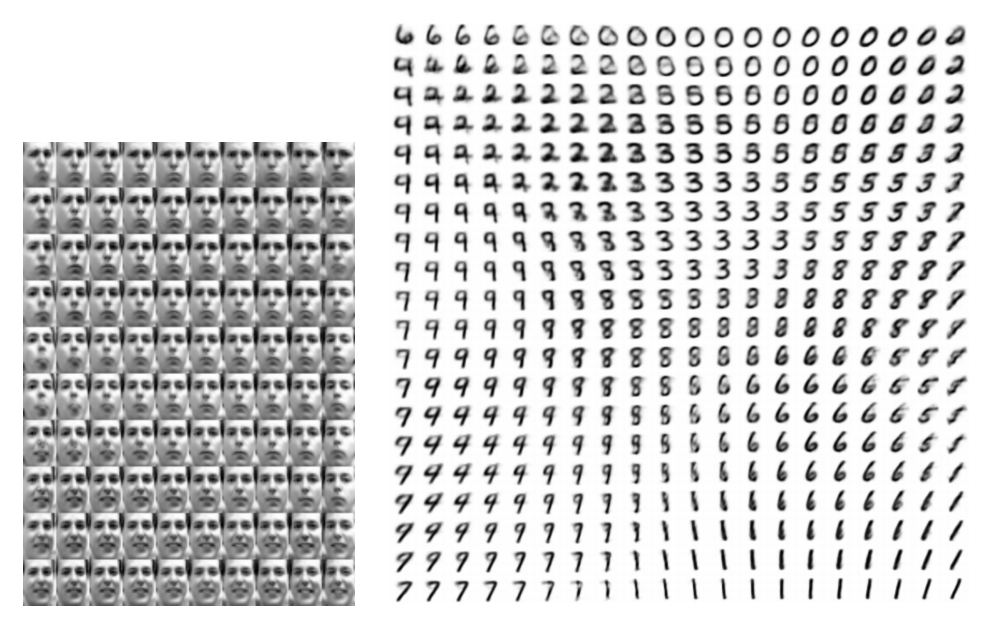
\includegraphics[width=\linewidth]{./figures/vae.png}
    \caption[VAEを用いて生成された画像の例]{VAEを用いて生成された画像の例(\cite{kingma2013autoencoding}より引用)}
    \label{fig:vae_example}
  \end{center}
\end{figure}

\clearpage
\section{深層状態空間モデル(DSSM)}
\label{section:dssm}

深層状態空間モデル(Deep State Space Model: DSSM, Deep Karman Filters, Deep Markov Model,単にSSMなどとも呼ばれる)\cite{krishnan2015deep}\cite{krishnan2017structured}について説明する.VAEがデータ一つ一つの潜在表現を考えるのに対し,DSSMは時間変化があるデータの各時刻の潜在表現を考えて更にその潜在表現の時間変化をモデル化したものであり,VAEを時系列方向に拡張したモデルとみなすこともできる.DSSMではこの潜在表現のことを状態表現と呼ぶ.

DSSMは特に深層強化学習の分野で用いられており,エージェントがある環境中で行動を起こした結果として視覚フィードバックや報酬フィードバックなどが得られるときに,DSSMで将来の観測を正しく予測できるよう学習することで良い環境の状態表現を獲得することができ,さらにその状態表現を用いることで良い行動方策が得られる\cite{hafner2019dream}.

\vspace{\baselineskip}
本論文では図 \ref{fig:ssm}のようなグラフィカルモデルで表されるDSSMのモデルを考えるが,行動系列が与えられない場合や,強化学習のように環境の状態に応じて報酬が与えられる問題においても以下の説明は同様にして考えることができる.

\begin{figure}[bp]
  \begin{center}
    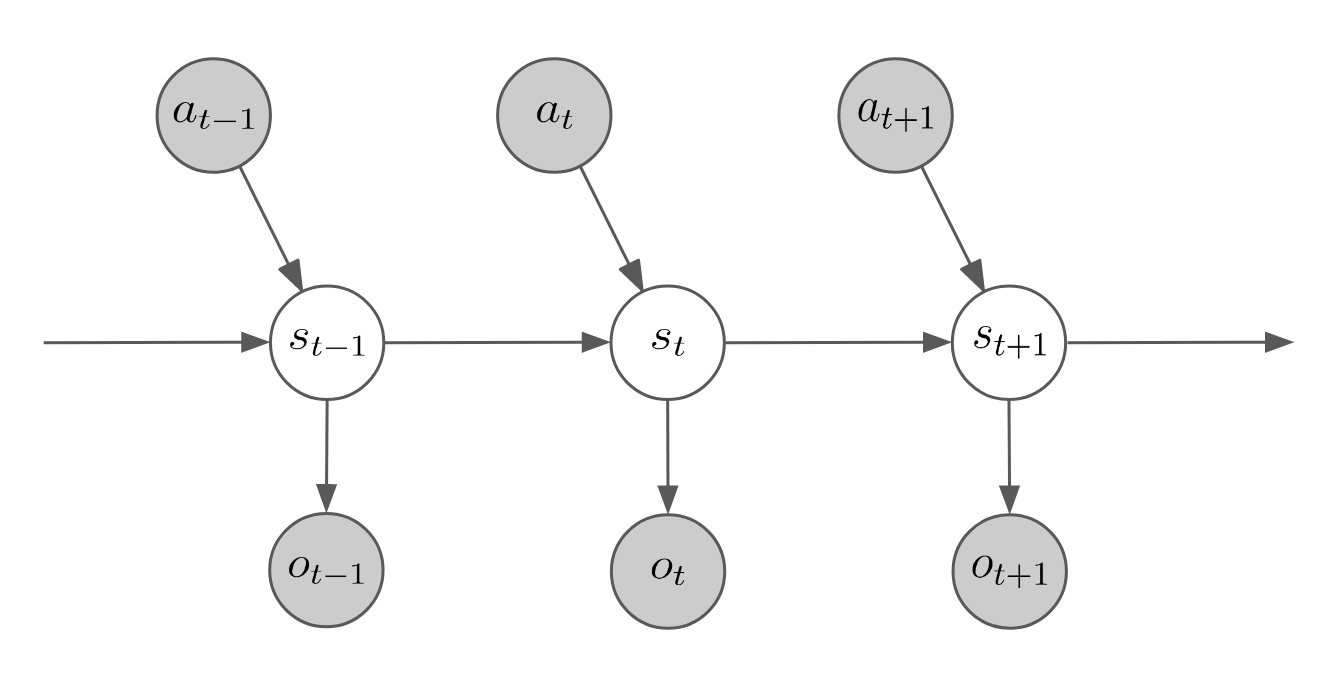
\includegraphics[width=\linewidth]{./figures/dssm.png}
    \caption{SSMのグラフィカルモデル}
    \label{fig:ssm}
  \end{center}
\end{figure}

\vspace{\baselineskip}
ここからDSSMの理論的な説明を行う.DSSMは式(\ref{eq:dssm})式が示すように,初期状態$s_0$と行動系列$a_{1:T}$で条件付けられた観測$o_{1:T}$を予測するモデルである.DSSMでは各時刻の観測$o_t$は各時刻の状態表現$s_t$から生成されると考え,各時刻の状態表現$s_t$を明示的に推論する.初期状態$s_0$の定め方は任意だが,多くの場合ゼロベクトルが用いられる.以降,簡単のため条件$s_0$は省略する.

\begin{eqnarray}
  p(o_{1:T}|a_{1:T}, s_0)
  &=& \prod_{t=1}^T p(o_t|a_{1:t}, s_0) \nonumber \\
  &=& \prod_{t=1}^T \int p(o_t|s_t) p(s_t|s_{t-1}, a_t)ds_t \label{eq:dssm}
\end{eqnarray}

DSSMでは以下の仮定をおく.式(\ref{eq:dssm_pre})は各時刻の状態ベクトル$s_t$は正規分布に従うという仮定で,式(\ref{eq:dssm_post})は$o_t$で条件付けられた各時刻の状態ベクトル$s_t$も正規分布に従うという仮定である.

\begin{eqnarray}
  p(s_t|s_{t-1}, a_t) &=& \mathcal{N}(s_t|\mu(s_{t-1}, a_t),\sigma(s_{t-1}, a_t))\label{eq:dssm_pre} \\
  p(s_t|s_{t-1}, a_t, o_t) &=& \mathcal{N}(s_t|\mu(s_{t-1}, a_t, o_t),\sigma(s_{t-1}, a_t, o_t))\label{eq:dssm_post}
\end{eqnarray}

さらにDSSMではVAEと同様に$s_t$の推論モデル$q(s_t|s_{t-1}, a_t, o_t)$を導入し,生成過程と推論モデルをニューラルネットによってモデル化し,最尤推定によってそれらのパラメータを求める.

以下の変分下限で最尤推定を行う.

\begin{eqnarray}
  \log p(o_{1:T}|a_{1:T})
  &=& \log \prod_{t=1}^T p(o_t|a_{1:t}) \nonumber \\
  &=& \log \prod_{t=1}^T \int p(o_t|s_t) p(s_t|s_{t-1}, a_t)ds_t \nonumber \\
  &=& \sum_{t=1}^T \log \int p(o_t|s_t) p(s_t|s_{t-1}, a_t)ds_t \nonumber \\
  &=& \sum_{t=1}^T \log \int q(s_t|s_{t-1}, a_t, o_t) \frac{p(o_t|s_t) p(s_t|s_{t-1}, a_t)}{q(s_t|s_{t-1}, a_t, o_t)}ds_t \label{eq:dssm_replace} \\
  &\geq& \sum_{t=1}^T \int q(s_t|s_{t-1}, a_t, o_t) \log \frac{p(o_t|s_t) p(s_t|s_{t-1}, a_t)}{q(s_t|s_{t-1}, a_t, o_t)}ds_t \label{eq:dssm_jensen} \\
  &=& \sum_{t=1}^T \left( \int q(s_t|s_{t-1}, a_t, o_t) \log p(o_t|s_t)ds_t \right. \nonumber \\
  && \hspace{2em} \left. - \int q(s_t|s_{t-1}, a_t, o_t) \log \frac{p(s_t|s_{t-1}, a_t)}{q(s_t|s_{t-1}, a_t, o_t)}ds_t \right) \nonumber \\
  &=& \sum_{t=1}^T \left( \mathbb{E}_{s_t \sim q(s_t|s_{t-1}, a_t, o_t)} [\log p(o_t|s_t)] \right. \nonumber \\
  && \hspace{2em} \left. - \mathbb{E}_{s_{t-1} \sim q(s_{t-1}|s_{t-2}, a_{t-1}, o_{t-1})} [\mathrm{D_{KL}}(q(s_t|s_{t-1}, a_t, o_t) \| p(s_t|s_{t-1}, a_t, o_t))] \right) \nonumber \\
  \label{eq:dssm_elbo}  
\end{eqnarray}

式(\ref{eq:dssm_jensen})にはイェンセンの不等式を用いている.式(\ref{eq:dssm_replace})では,$s_t$の周辺化を排除するために先述した近似分布$q(s_t|s_{t-1}, a_t, o_t)$を導入し,さらに式(\ref{eq:dssm_elbo})で$s_t$, $s_{t-1}$をサンプリングしてモンテカルロ近似を行う.
式(\ref{eq:dssm_elbo})の第2項のカルバックライブラー距離は,いま$p(s_t|s_{t-1}, a_t, o_t))$,$q(s_t|s_{t-1}, a_t, o_t)$共にガウス分布を仮定しているため,解析的に計算することができ,また式(\ref{eq:elbo})の第1項は,$p(o_t|s_t)$の分布に正規分布やベルヌーイ分布を仮定することで尤度が計算できる.

この変分下限を目的関数にすることで各モデルを学習することができる.また学習時には10フレーム程度先までの予測を行うのが一般的であるが,学習時の予測の長さとモデルの評価時の予測の長さを揃える必要はなく,評価時にはより長期の予測も可能である.

最後に$s_0$の求め方について,初期状態が必ず一定な問題設定ではゼロベクトルなど一定の値に決め打ちすることができるが,様々な初期状態が考えられる場合は何らかの方法で推論する必要がある.本研究では慣例に習って$s_0$を$s_0 \sim q(s_0|\vec{0}, \vec{0}, o_0) $によって定め,(\ref{eq:dssm_elbo})の第2項の$s_0$のサンプリングは($o_{t=-1}$や$a_{t=-1}$が与えられない前提を考えるため)これで置き換える.$s_0$の推論方法については議論の余地があると考えられ,これについては考察「初期状態の推論」で触れる.

\vspace{\baselineskip}
以上がDSSMの概要である.DSSMを用いると,図 \ref{fig:dssm_dkf},図 \ref{fig:dssm_planet} のように数フレーム先を予測することができる.図 \ref{fig:dssm_dkf}は,行動系列として回転情報が与えられており,回転する画像の予測を行う.図 \ref{fig:dssm_planet}は四足歩行するシミュレータ上のエージェントの第三者視点からの観測を予測しており,行動系列としてエージェントの各関節に加えられる力が与えられている.DSSMは長期の予測をした際にも生成自体が安定している点で自己回帰モデルと比較して優れている.

% \caption[hoge]{fuga}
\begin{figure}[bp]
  \begin{center}
    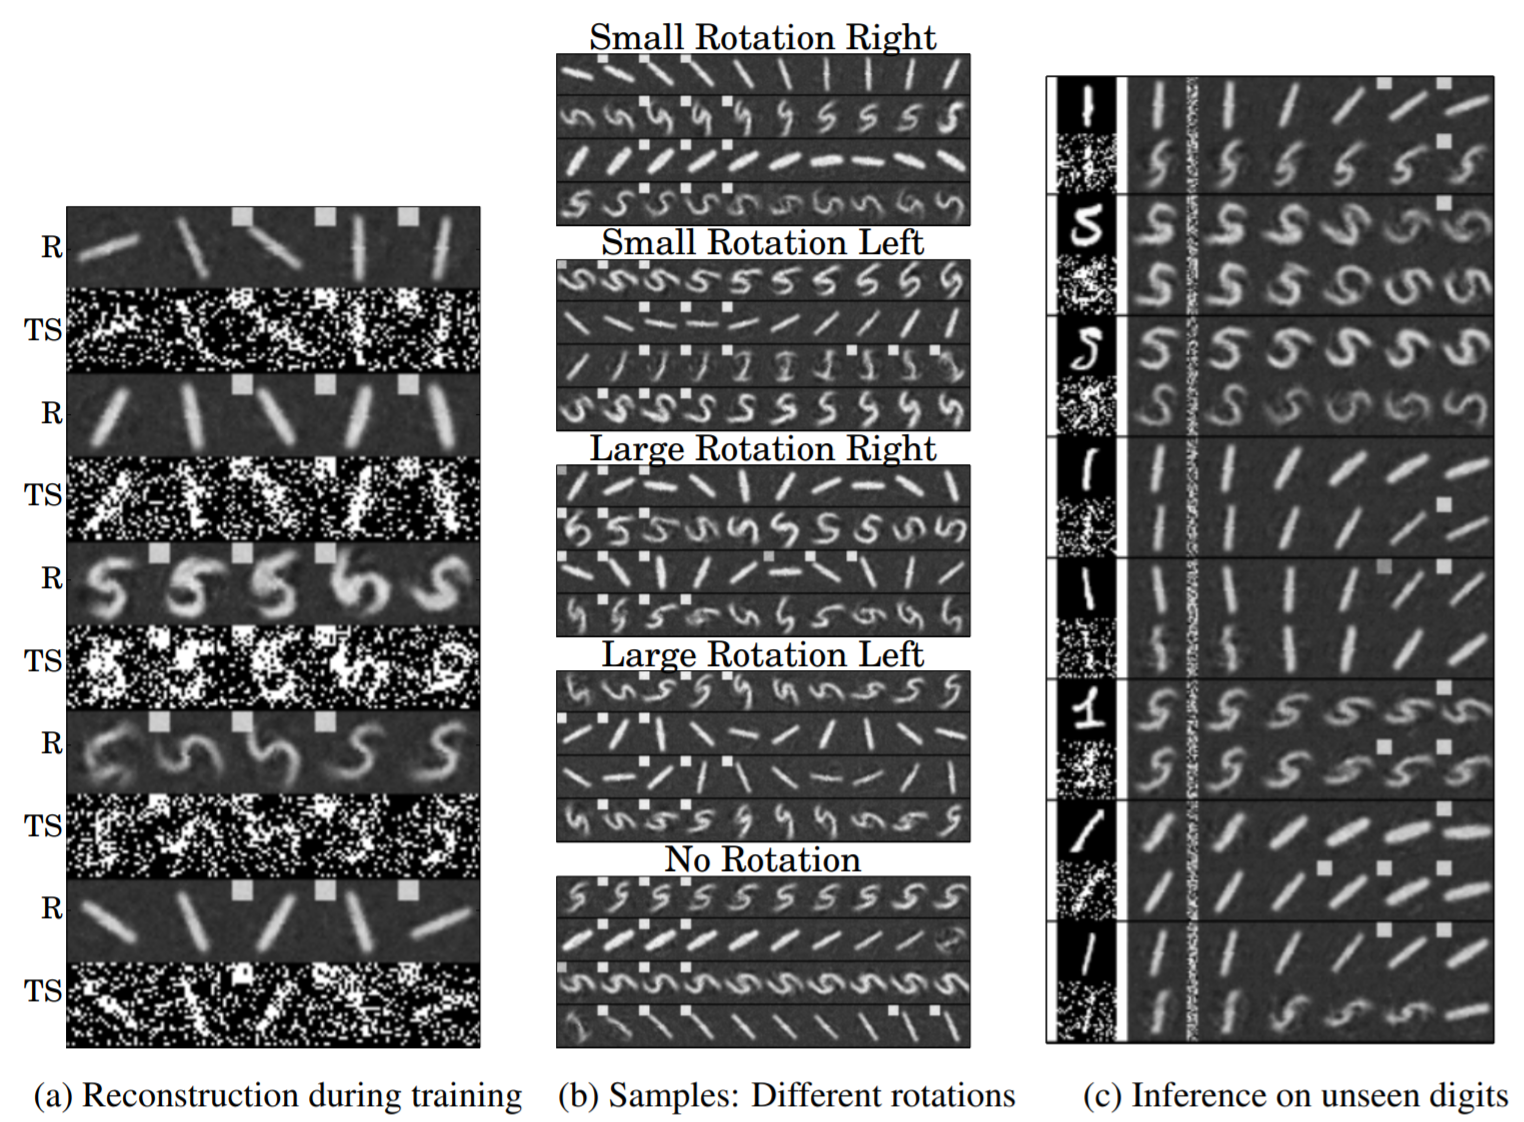
\includegraphics[width=\linewidth]{./figures/dssm_dkf.png}
    \caption[DSSMで生成される映像の例(回転する数字画像)]{DSSMで生成される映像の例(回転する数字画像).\cite{krishnan2015deep}より引用}
    \label{fig:dssm_dkf}
  \end{center}
\end{figure}

% \caption[hoge]{fuga}
\begin{figure}[tbp]
  \begin{center}
    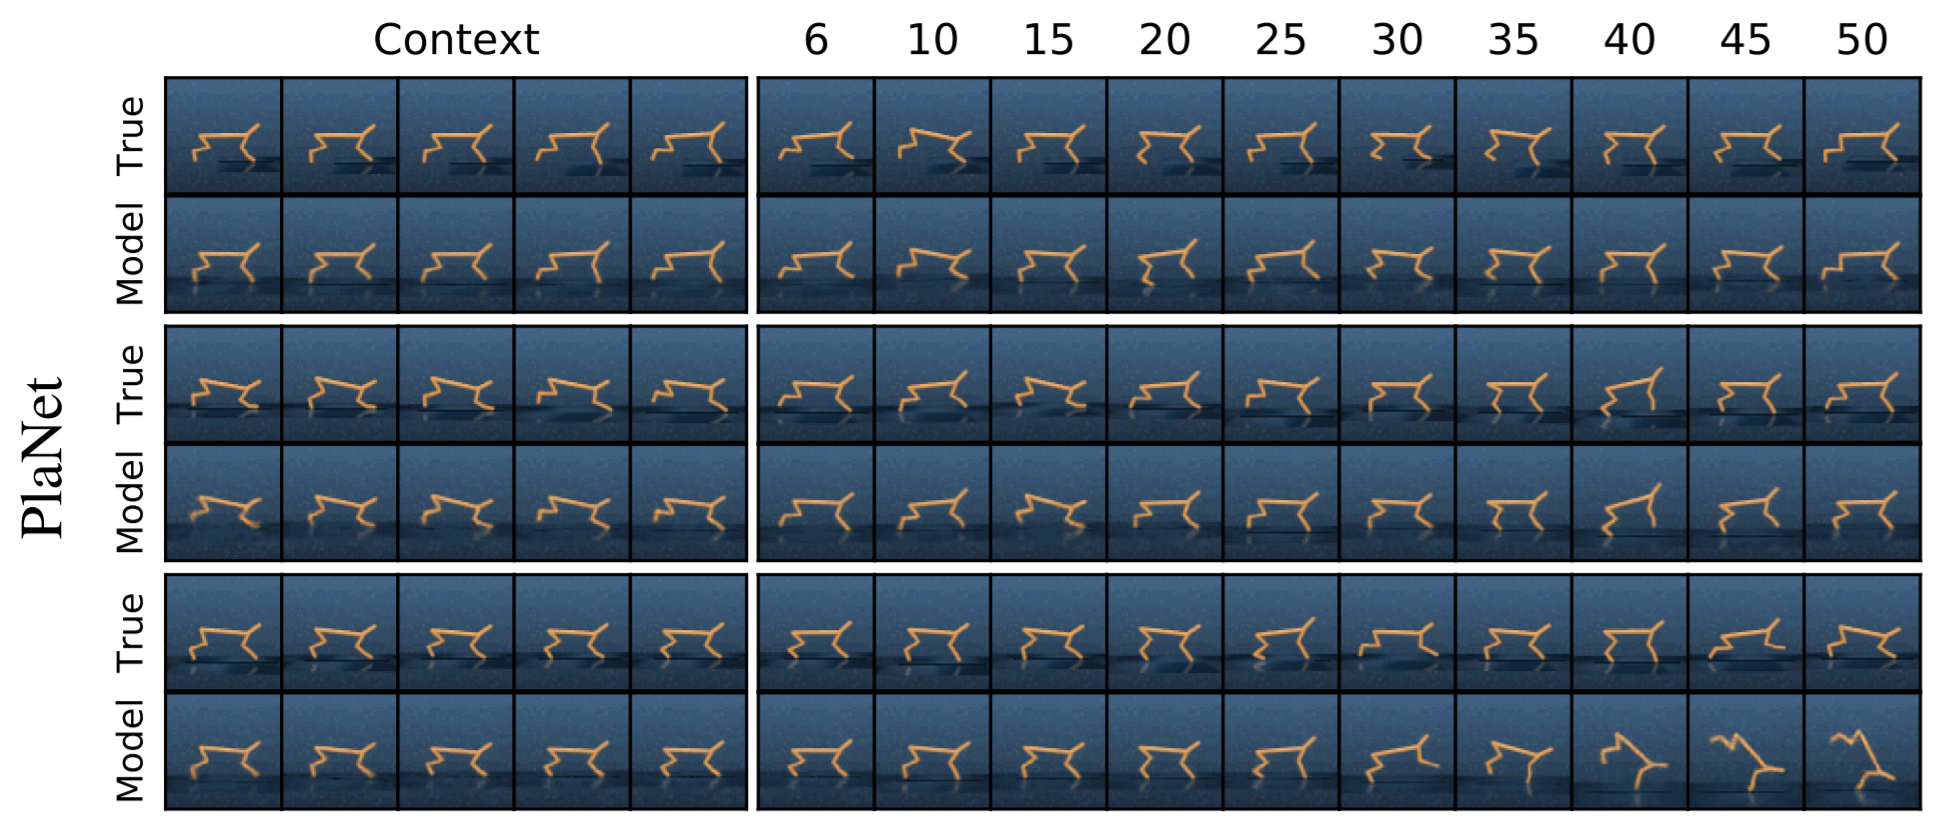
\includegraphics[width=\linewidth]{./figures/dssm_planet.png}
    \caption[DSSMで生成される映像の例(強化学習エージェント)]{DSSMで生成される映像の例(強化学習エージェント).\cite{hafner2019planet}より引用}
    \label{fig:dssm_planet}
  \end{center}
\end{figure}

